

---- TODO ---- \\

Co i dlaczego tak w sumie budujemy? \\

Jedną z najważniejszych decyzji w trakcie realizacji projektu był wybór rodzaju kości, jaką miał odczytywać 
i interpretować model sztucznej inteligencji.
Jako najistotniejsze kryterium wyznaczono liczbę ścian będącą potęgą liczby dwa
(już na wstępnym etapie projektowania odrzucając standardową kość sześciościenną) --
w celu łatwej interpretacji wyniku w notacji binarnej, stosowanej powszechnie w informatyce oraz kryptografii.
W następnej kolejności szukano kompromisu pomiędzy łatwością w odczycie ścianek a generowaniem jak największej liczby
bitów jednym rzutem -- czyli kości o jak największej liczbie ścianek.

Z dostępnych powszechnie na rynku kości tylko cztero-, ośmio- i szesnastościenne spełniają pierwszy z wymienionych wyżej kryteriów.
Kość czterościenną odrzucono początkowo ze względu na jej kształt ostrosłupa foremnego o podstawie trójkąta,
na której liczby zapisywane są na rogach a nie ściankach (co pokazano na rysunku~\ref{fig:k4}),
jednak powróciła ona do dyskusji w postaci niestandardowych kształtów kości, które pokazano na rysunku~\ref{fig:nietypowe_modern_k4}.
Niestety nie na długo, z racji na bardzo niską dostępność na runku tego typu kości, oraz rzucające się w oczy problemy
z odczytywaniem pustych (zaokrąglonych) ścianek kości typu modern, pokazanych na rysunku~\ref{fig:modern_k4},
oraz takich z bardzo małymi oznaczeniami, które przestałyby być widoczne przy nawet niewielkim przechyleniu kości
dla ściętego ostrosłupa pokazanych na rysunku~\ref{fig:nietypowe_k4}.

Kość szesnanstościenną również odrzucono ze względu na mały rozmiar ścianek, który sprawia,
że na zdjęciu robionym idealnie nad kością widoczne jest kilka ścianek jednocześnie, jak pokazano na rysunku~\ref{fig:k16}.
Z pozostałych opcji tylko na kości ośmiościennej (pokazanej na rysunku~\ref{fig:k8}) widać z góry dokładnie jedną ściankę,
a do tego ma liczbę ścianek będącą potęgą 2, zatem to ten rodzaj kości został wybrany do użycia w projekcie.

\begin{figure}[h]
    \centering
      \begin{subfigure}{.3\textwidth}
        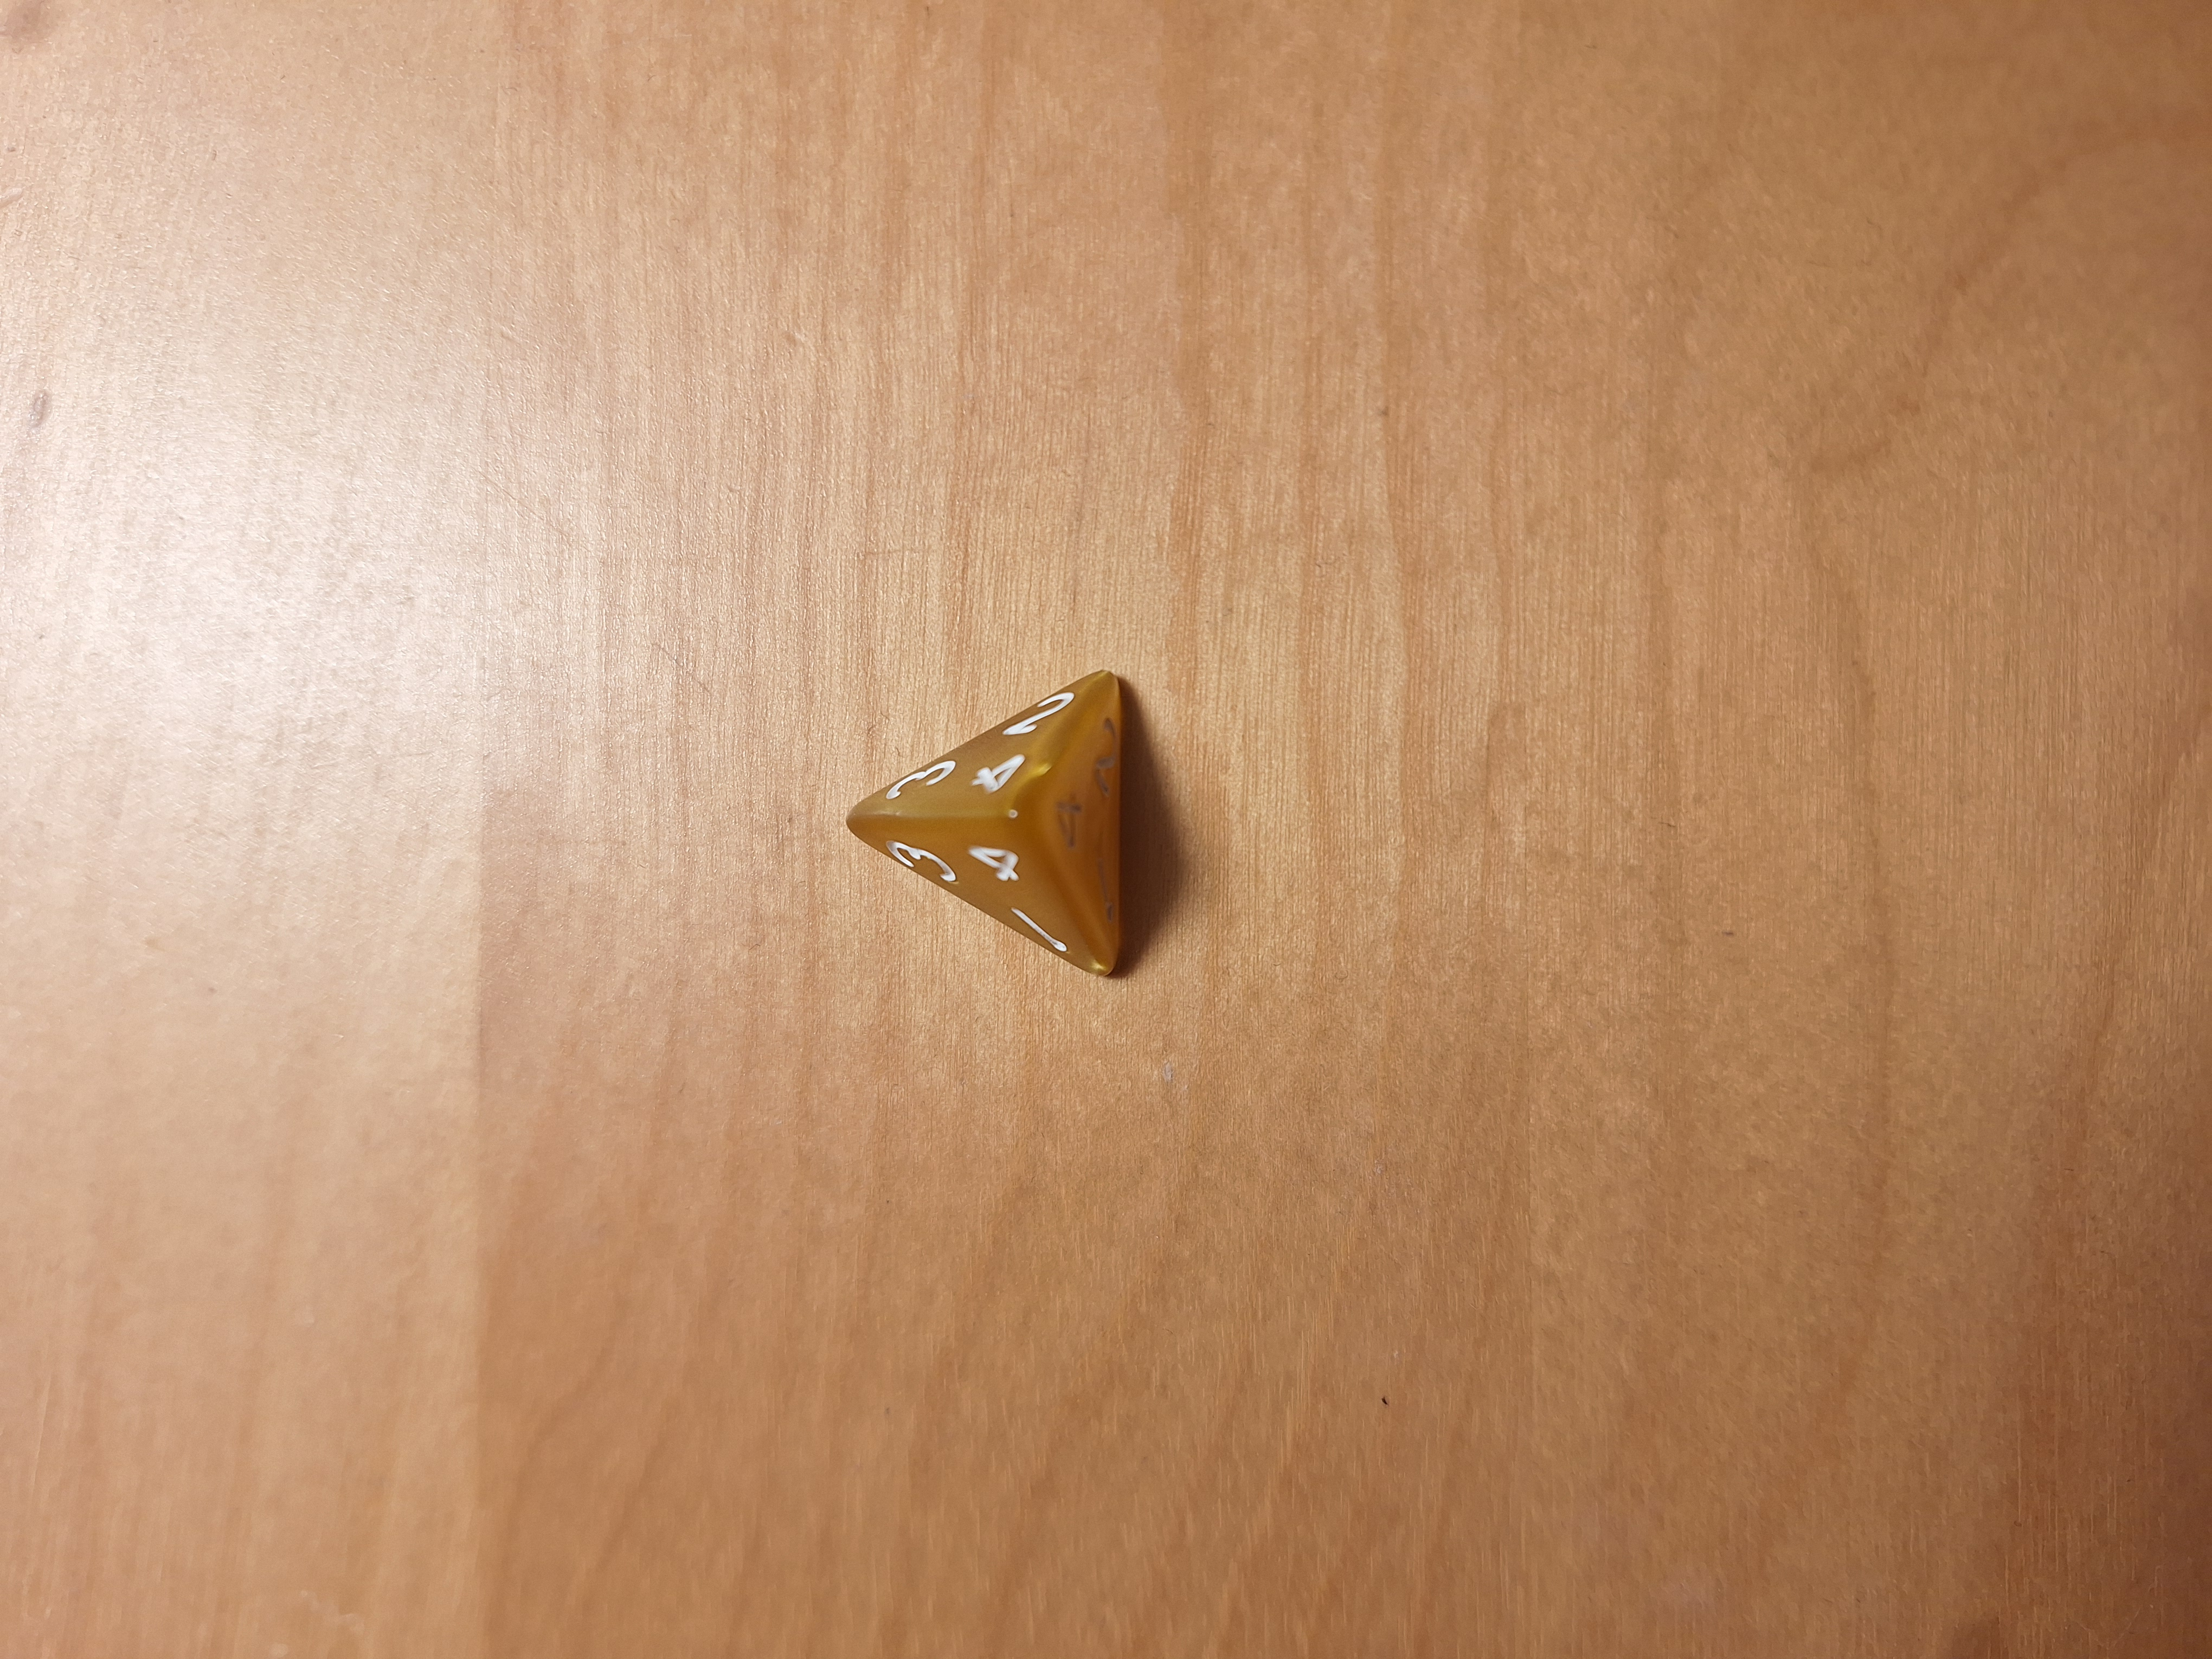
\includegraphics[width=.9\linewidth, trim={250mm 200mm 350mm 150mm}, clip]{chapters/02-teoria/figures/k4}
        \caption{\label{fig:k4}Kość czterościenna}
      \end{subfigure}%
      \begin{subfigure}{.3\textwidth}
        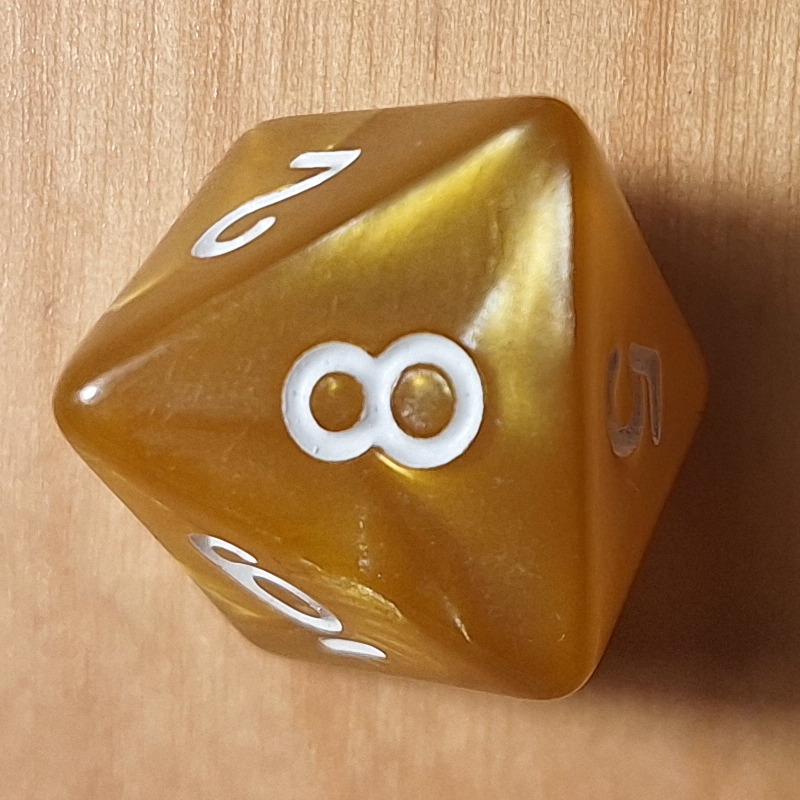
\includegraphics[width=.9\linewidth, trim={250mm 200mm 350mm 150mm}, clip]{chapters/02-teoria/figures/k8}
        \caption{\label{fig:k8}Kość ośmiościenna}
      \end{subfigure}%
       \begin{subfigure}{.3\textwidth}
        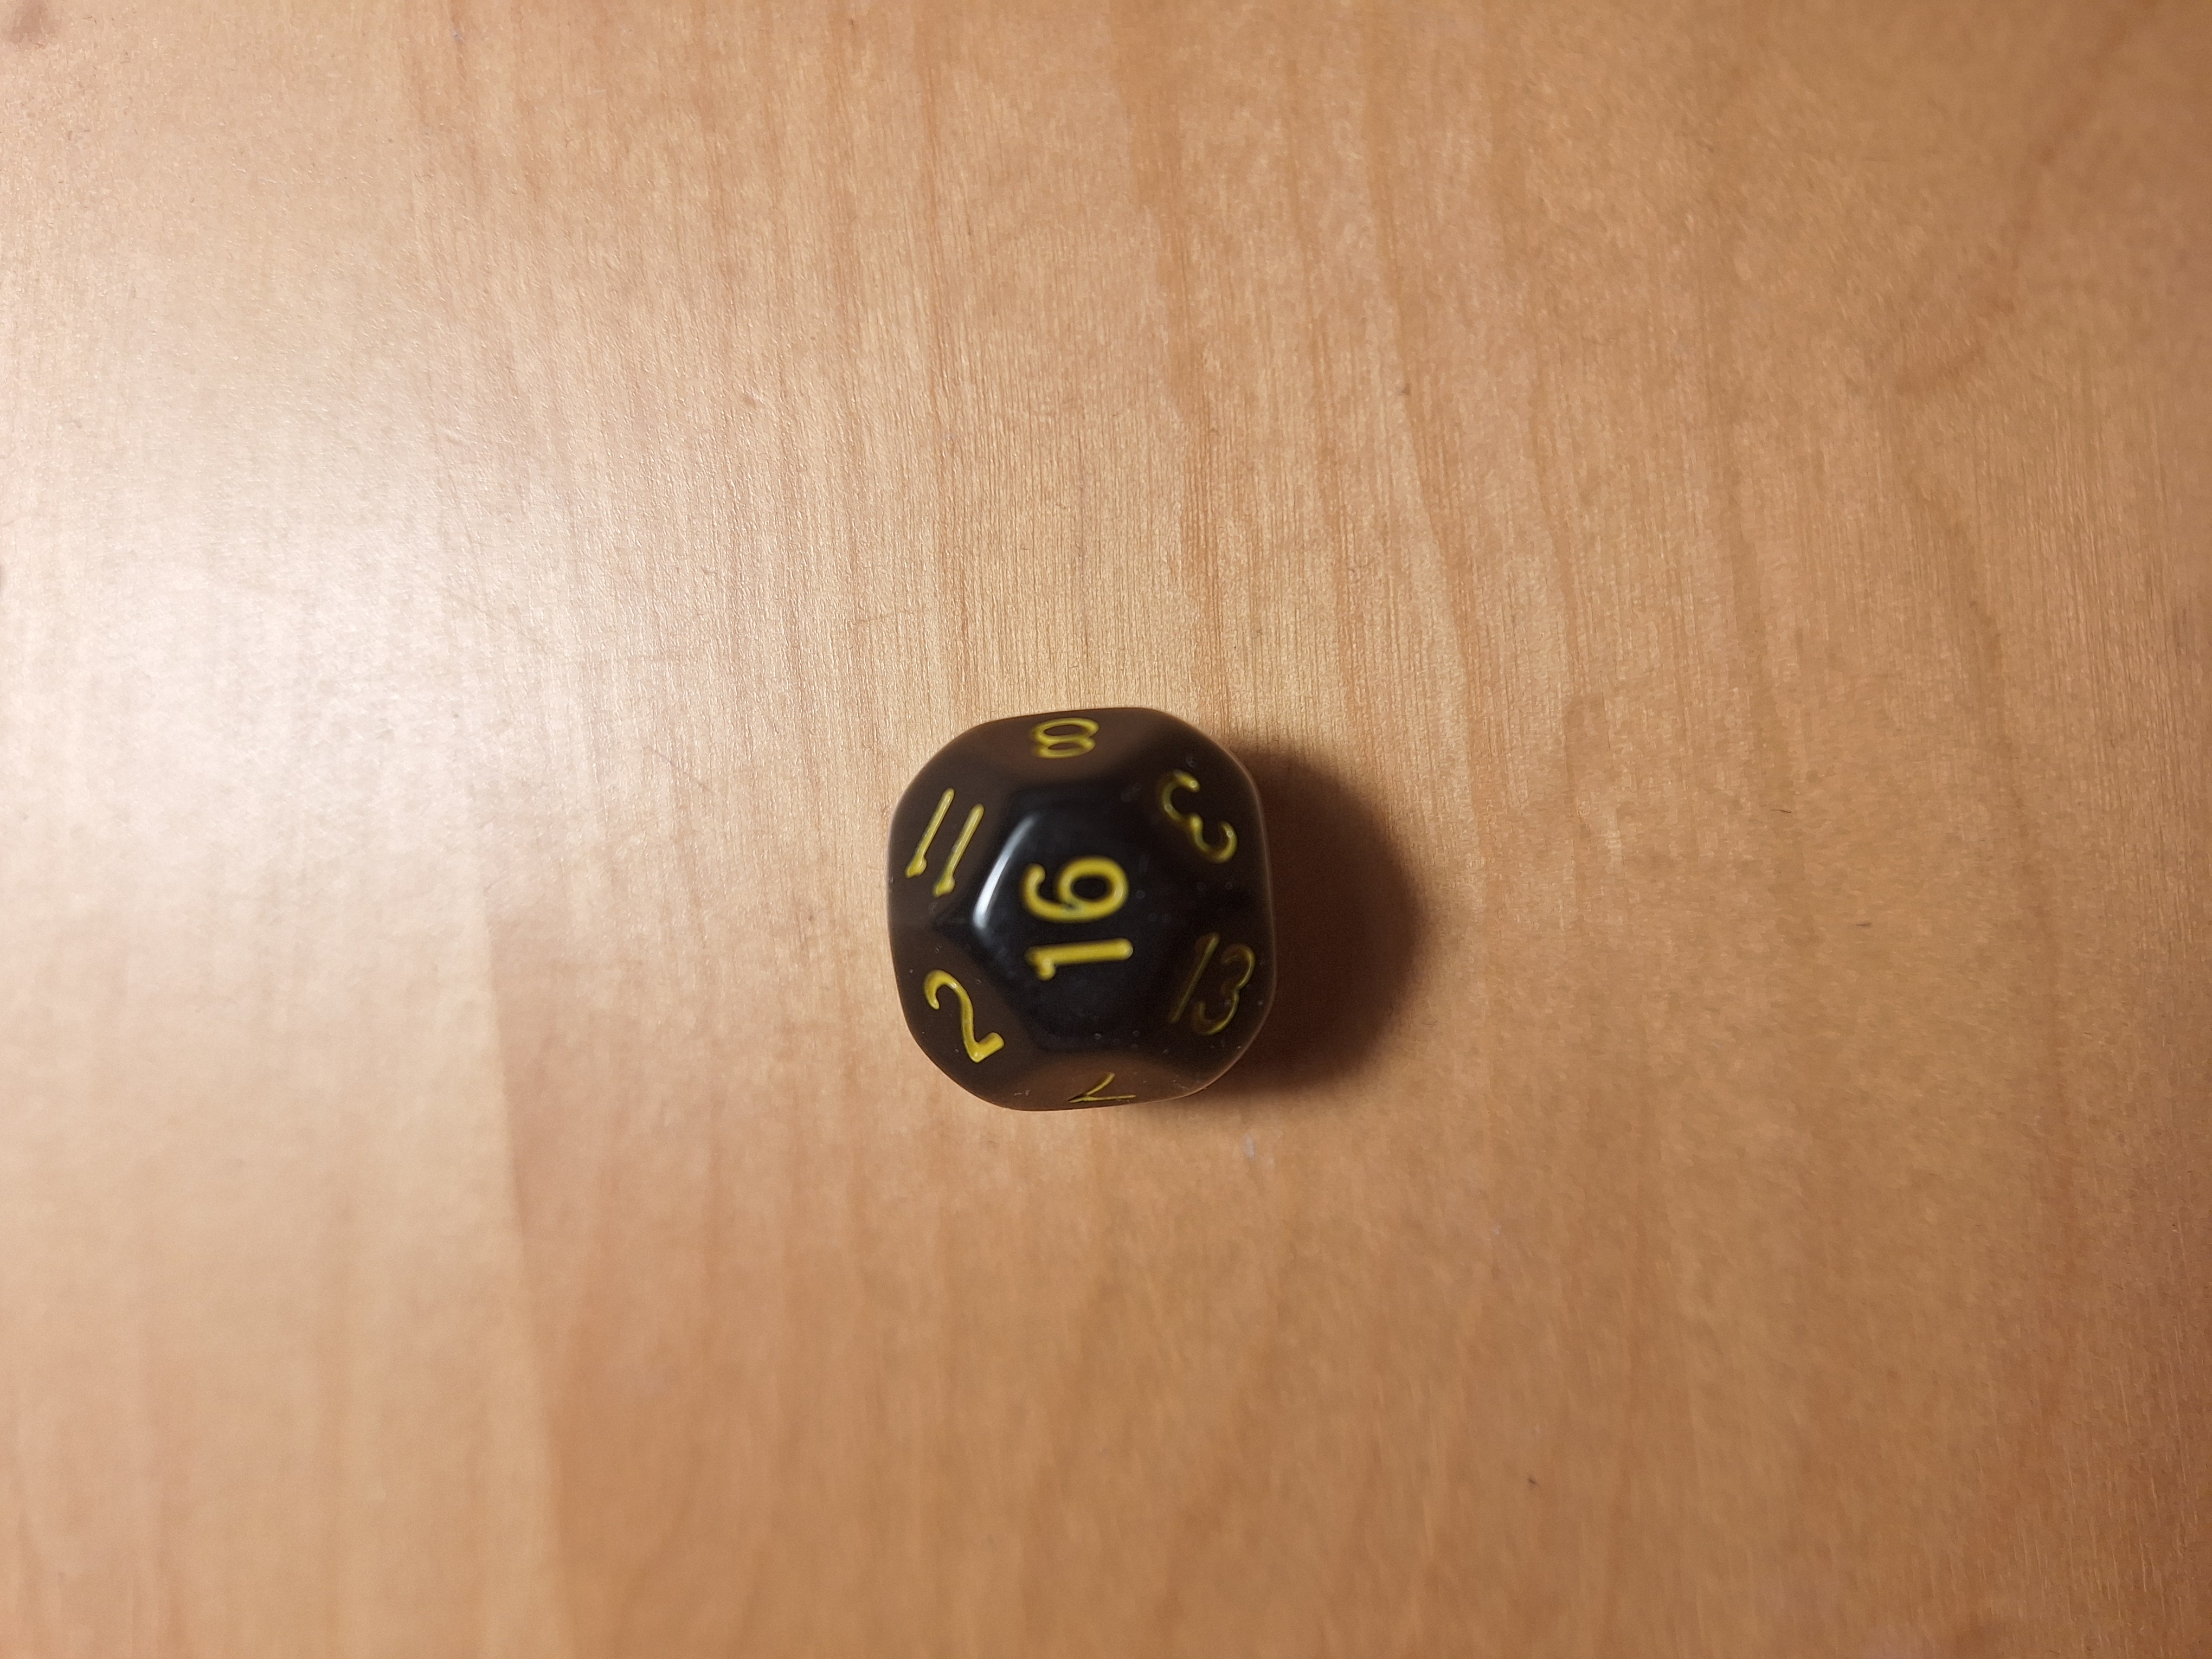
\includegraphics[width=.9\textwidth, trim={300mm 150mm 300mm 200mm}, clip]{chapters/02-teoria/figures/k16}
        \caption{\label{fig:k16}Kość szesnastościenna}
      \end{subfigure}
    \caption{Zdjęcia kości z góry}
\end{figure}

\begin{figure}[h]
    \centering
      \begin{subfigure}{.45\textwidth}
        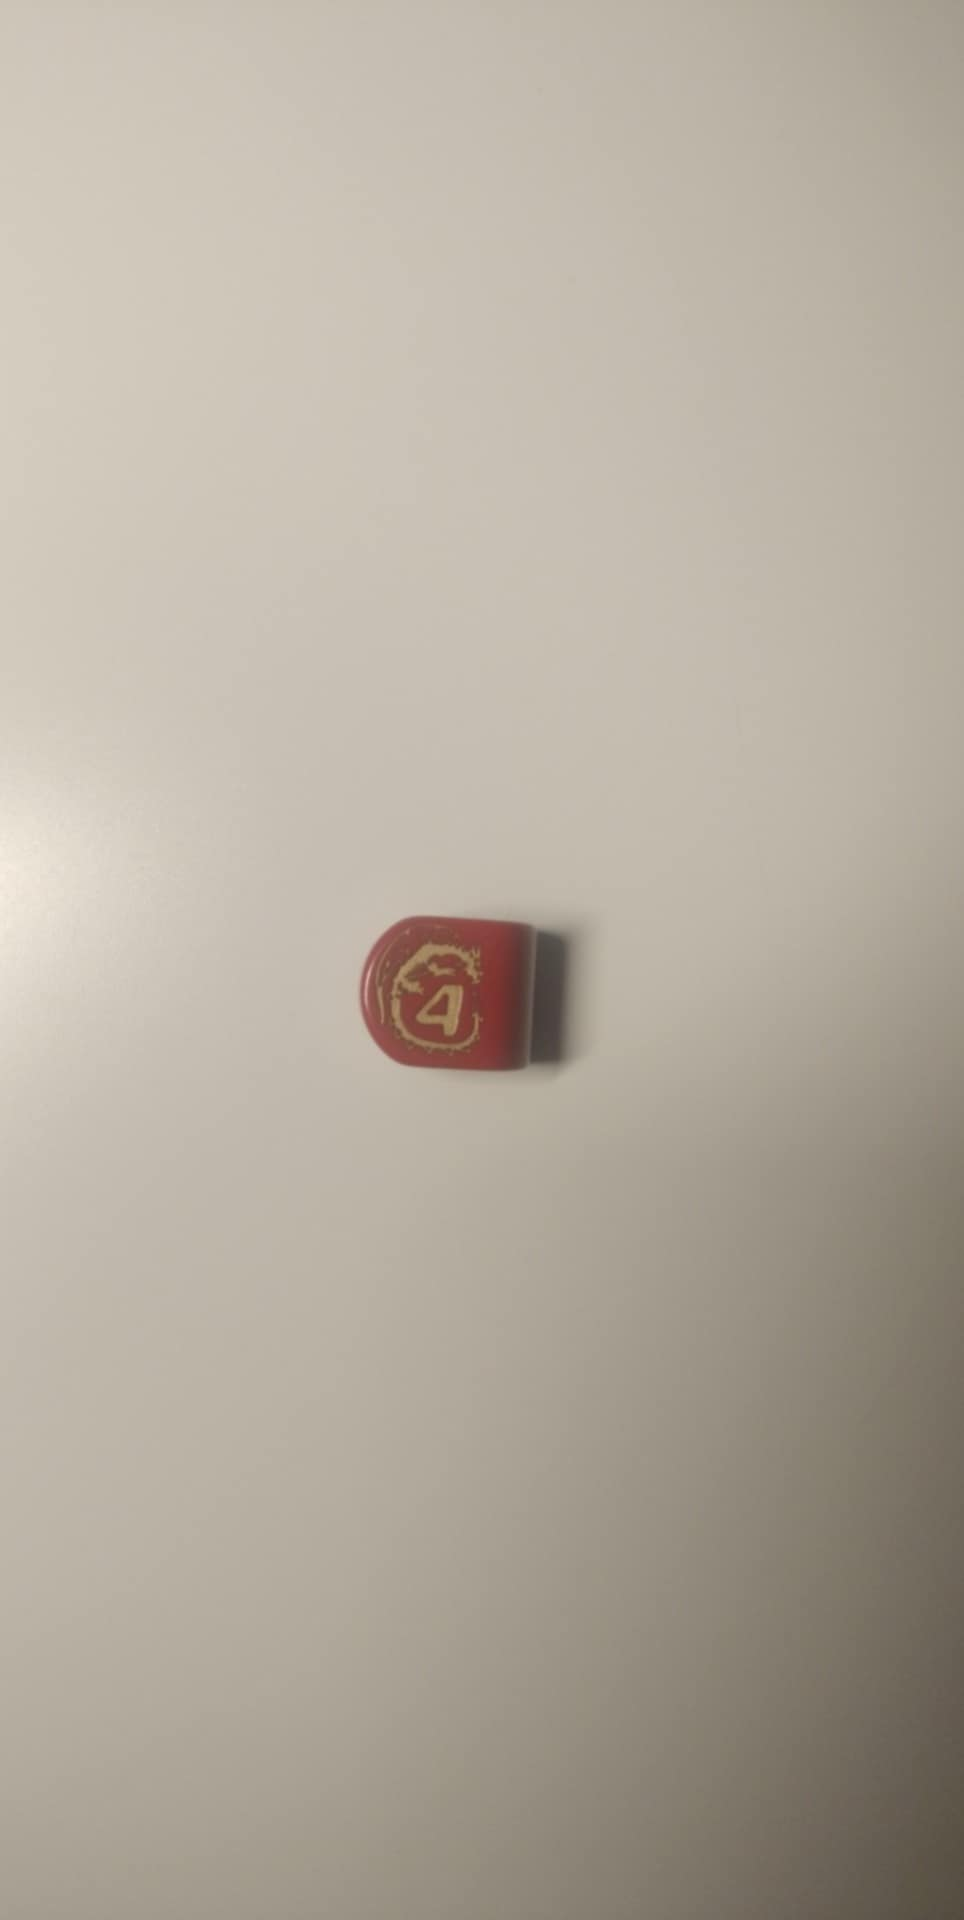
\includegraphics[width=.9\linewidth]{chapters/02-teoria/figures/modern_k4}
        \caption{\label{fig:modern_k4}Kość czworościenna typu „modern”}
      \end{subfigure}%
      \begin{subfigure}{.45\textwidth}
        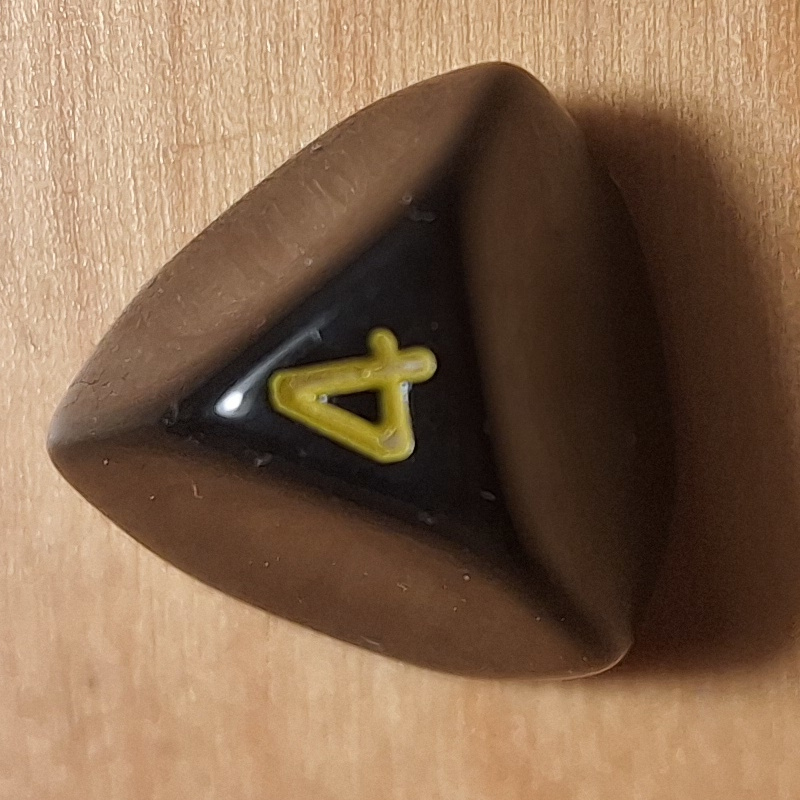
\includegraphics[width=.9\linewidth, trim={250mm 200mm 350mm 150mm}, clip]{chapters/02-teoria/figures/nietypowe_k4}
        \caption{\label{fig:nietypowe_k4}Kość czworościenna ze ściętym czubkiem}
      \end{subfigure}%
    \caption{Nietypowe kości czworościenne}
    \label{fig:nietypowe_modern_k4}
\end{figure}